\documentclass[11pt,a4paper]{article}

\usepackage[utf8]{inputenc}
\usepackage[T1]{fontenc}
\usepackage{mathpazo}
\usepackage[scaled=0.92]{helvet}
\usepackage[margin=1in]{geometry}
\usepackage{graphicx}
\usepackage{amsmath,amssymb,amsfonts}
\usepackage{booktabs}
\usepackage{tabularx}
\usepackage{setspace}
\usepackage{titlesec}
\usepackage{fancyhdr}
\usepackage{float}
\usepackage{caption}

\usepackage{tikz}
\usetikzlibrary{shapes.geometric, arrows.meta, positioning, calc, shadows, backgrounds}
\usepackage[hidelinks]{hyperref}

\setstretch{1.15}
\setlength{\parindent}{0pt}
\setlength{\parskip}{8pt}
\sloppy

\titleformat{\section}{\normalfont\large\bfseries\sffamily}{\thesection}{1em}{}
\titleformat{\subsection}{\normalfont\normalsize\bfseries\sffamily}{\thesubsection}{1em}{}

\pagestyle{fancy}
\fancyhf{}
\fancyhead[L]{\small\sffamily Analisis Pemodelan Data: Entity Relationship Diagram}
\fancyhead[R]{\small\sffamily\thepage}
\renewcommand{\headrulewidth}{0.4pt}

\captionsetup{font=small,labelfont=bf,labelsep=period}

\renewenvironment{abstract}
{\small
	\begin{center}\textbf{\sffamily Abstract}\end{center}
	\begin{quote}}
	{\end{quote}}

\title{\vspace{-1.5cm}\textbf{\sffamily\LARGE Analisis Pemodelan Data: \\ Entity Relationship Diagram (ERD)}}
\author{
	\textbf{Muhammad Riduwan Khafidi} \\
	\small Program Studi Teknik Rekayasa Perangkat Lunak \\
	\small Politeknik Negeri Batam \\
	\small \texttt{4342611034@students.polibatam.ac.id}
}
\date{\small\today}

\begin{document}

\maketitle
\thispagestyle{empty}

\begin{abstract}
	Perancangan basis data berskala besar tidak dapat dilakukan secara instan. Perancang seringkali dihadapkan pada kompleksitas kebutuhan pengguna yang sulit diterjemahkan langsung ke dalam tabel fisik. Untuk menjembatani celah ini, digunakanlah Entity Relationship Diagram (ERD) sebagai model konseptual. ERD memvisualisasikan entitas (objek dunia nyata), atribut (properti entitas), dan relasi (hubungan antar entitas) secara intuitif. Makalah ini membedah secara komprehensif seluruh anatomi ERD, mulai dari notasi dasar, jenis-jenis atribut, hirarki kunci (keys), derajat relasi, kardinalitas, batasan partisipasi, hingga konsep entitas lemah (weak entity). Pemahaman mendalam terhadap ERD merupakan fondasi mutlak sebelum skema konseptual ini dipetakan menjadi skema relasional yang siap diimplementasikan ke dalam DBMS.
\end{abstract}

\section{Mengapa Kita Membutuhkan ERD?}

Bayangkan seorang arsitek yang akan membangun gedung pencakar langit. Ia tidak akan langsung menyuruh tukang untuk menyusun batu bata. Ia harus menggambar blueprint (cetak biru) terlebih dahulu. Begitu pula dalam pembuatan basis data. Pada skala kecil, perancang mungkin bisa langsung memutuskan struktur tabelnya. Namun, pada aplikasi berskala besar, seringkali tidak ada satu orang pun yang memahami secara menyeluruh data apa saja yang dibutuhkan.

Di sinilah Entity Relationship Diagram (ERD) berperan. ERD adalah teknik pemodelan data tingkat konseptual yang mengilustrasikan secara visual entitas dan relasi di dalam sebuah sistem. ERD bertindak sebagai bahasa universal yang menjembatani komunikasi antara perancang basis data dengan *customer* (pengguna). Melalui ERD, kita dapat memetakan integritas batasan (*integrity constraints*) dan aturan bisnis (*business rules*) sebelum menuliskan satu baris kode SQL pun.

\section{Anatomi Dasar: Entitas, Atribut, dan Relasi}

Sebuah ERD tersusun dari tiga komponen utama. Pertama adalah \textbf{Entitas} (\textit{Entity}), yaitu objek di dunia nyata yang dapat dibedakan dari objek lain, misalnya "Pegawai", "Departemen", atau "Mahasiswa". Dalam diagram, entitas digambarkan dengan persegi panjang. Kumpulan entitas yang serupa disebut \textit{Entity Set}, dan setiap entitas set wajib memiliki kunci (\textit{key}).

Kedua adalah \textbf{Atribut}, yaitu properti yang melekat pada entitas. Misalnya, entitas "Pegawai" memiliki atribut "Nama", "Nomor Pegawai", dan "Tanggal Lahir". Sebuah atribut dilambangkan dengan elips.

Ketiga adalah \textbf{Relasi} (\textit{Relationship}), yaitu hubungan yang terjadi antar entitas, misalnya "Pegawai" bekerja di "Departemen". Relasi digambarkan dengan belah ketupat (\textit{diamond}). Sebuah relasi juga bisa memiliki atribut sendiri, seperti atribut "Mulai" yang menyimpan tanggal kapan seorang pegawai mulai bekerja di departemen tersebut.

\subsection{Tipe-Tipe Atribut}
Tidak semua atribut digambarkan dengan cara yang sama. Terdapat beberapa tipe atribut khusus yang penting untuk dipahami. Perhatikan Gambar \ref{fig:atribut} di bawah ini.

\begin{figure}[H]
	\centering
	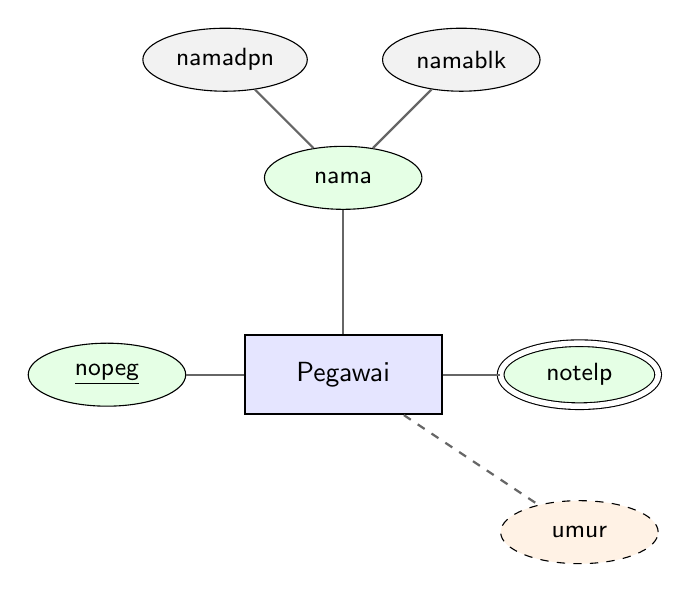
\begin{tikzpicture}[
			entity/.style={draw, rectangle, minimum width=2.5cm, minimum height=1cm, fill=blue!10, thick, font=\sffamily},
			attr/.style={draw, ellipse, minimum width=2cm, minimum height=0.8cm, fill=green!10, font=\small\sffamily},
			multi/.style={draw, ellipse, double, double distance=2pt, minimum width=2cm, minimum height=0.8cm, fill=green!10, font=\small\sffamily},
			derived/.style={draw, ellipse, dashed, minimum width=2cm, minimum height=0.8cm, fill=orange!10, font=\small\sffamily},
			link/.style={thick, color=gray!80!black}
		]
		\node[entity] (pegawai) at (0,0) {Pegawai};

		\node[attr] (nopeg) at (-3,0) {\underline{nopeg}};
		\draw[link] (pegawai) -- (nopeg);

		\node[multi] (notelp) at (3,0) {notelp};
		\draw[link] (pegawai) -- (notelp);

		\node[derived] (umur) at (3,-2) {umur};
		\draw[link, dashed] (pegawai) -- (umur);

		\node[attr] (nama) at (0,2.5) {nama};
		\node[attr, fill=gray!10] (namadpn) at (-1.5,4) {namadpn};
		\node[attr, fill=gray!10] (namablk) at (1.5,4) {namablk};
		\draw[link] (pegawai) -- (nama);
		\draw[link] (nama) -- (namadpn);
		\draw[link] (nama) -- (namablk);
	\end{tikzpicture}
	\caption{Ilustrasi Ragam Tipe Atribut pada Entitas Pegawai.}
	\label{fig:atribut}
\end{figure}

Atribut \textbf{Simple} (seperti \texttt{nopeg}) tidak dapat dipecah lagi. Atribut yang menjadi \textbf{Primary Key} (Kunci Utama) ditandai dengan garis bawah. Atribut \textbf{Composite} (seperti \texttt{nama}) dapat dipecah menjadi bagian yang lebih kecil (\texttt{namadpn} dan \texttt{namablk}). Atribut \textbf{Multi-valued} (seperti \texttt{notelp}) memungkinkan satu entitas memiliki lebih dari satu nilai, dilambangkan dengan elips garis ganda. Terakhir, atribut \textbf{Derived} (seperti \texttt{umur}) nilainya dihasilkan (diturunkan) dari atribut lain (seperti tanggal lahir), dilambangkan dengan elips garis putus-putus.

\section{Hirarki Kunci (Keys)}

Dalam basis data, tidak boleh ada dua entitas yang benar-benar identik. Oleh karena itu, kita membutuhkan sebuah Kunci (\textit{Key}) untuk membedakannya. Proses identifikasi kunci ini memiliki tahapan bertingkat.

Langkah pertama adalah \textbf{Superkey}, yaitu satu atau lebih atribut yang secara unik dapat membedakan setiap entitas. Dari superkey ini, kita memilih yang paling minimal (tanpa atribut mubazir) yang disebut \textbf{Candidate Key}. Terakhir, dari beberapa kandidat, kita memilih satu yang paling representatif sebagai \textbf{Primary Key} (Kunci Utama). Sebagai contoh, atribut \texttt{NIK} atau \texttt{NIM} biasanya dipilih sebagai Primary Key, bukan atribut \texttt{Nama}, karena nama bisa saja sama.

\section{Derajat Relasi dan Peran}

Relasi antar entitas memiliki tingkat kompleksitas yang disebut Derajat Relasi (\textit{Degree of Relationship}). Relasi paling sederhana adalah \textbf{Unary} (satu entitas berelasi dengan dirinya sendiri, misalnya Pegawai memiliki atasan sesama Pegawai). \textbf{Binary} adalah relasi antara dua entitas (Pegawai dengan Departemen). Sedangkan \textbf{Ternary} melibatkan tiga entitas sekaligus, seperti pada Gambar \ref{fig:ternary}.

\begin{figure}[H]
	\centering
	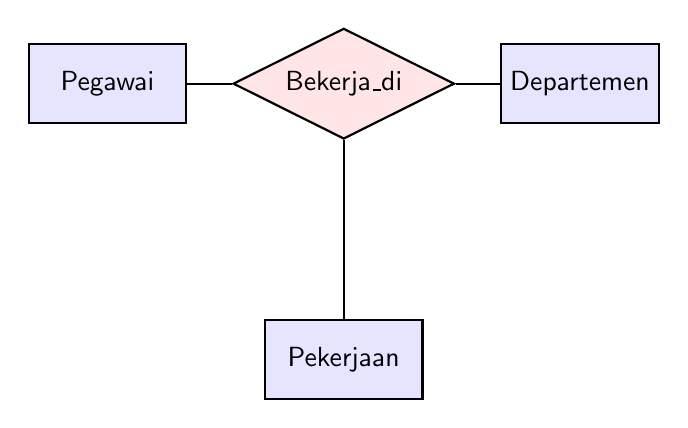
\begin{tikzpicture}[
			entity/.style={draw, rectangle, minimum width=2cm, minimum height=1cm, fill=blue!10, thick, font=\sffamily},
			relation/.style={draw, diamond, aspect=2, minimum width=2.5cm, minimum height=1cm, fill=red!10, thick, font=\sffamily}
		]
		\node[entity] (pegawai) at (0,2) {Pegawai};
		\node[entity] (dept) at (6,2) {Departemen};
		\node[entity] (job) at (3,-1.5) {Pekerjaan};
		\node[relation] (kerja) at (3,2) {Bekerja\_di};

		\draw[thick] (pegawai) -- (kerja);
		\draw[thick] (dept) -- (kerja);
		\draw[thick] (job) -- (kerja);
	\end{tikzpicture}
	\caption{Relasi Ternary antara Pegawai, Departemen, dan Pekerjaan.}
	\label{fig:ternary}
\end{figure}

Selain derajat, entitas yang sama dapat memiliki peran (\textit{role}) yang berbeda. Contoh klasiknya adalah relasi \textit{Bertanggung\_jawab\_pada} antar entitas Pegawai. Di sini, Pegawai berperan sebagai "Supervisor" bagi pegawai lainnya, dan berperan sebagai "Bawahan" bagi supervisor tersebut.

\section{Kardinalitas (Cardinality)}

Kardinalitas mendefinisikan jumlah maksimum entitas yang dapat diasosiasikan dengan entitas lain melalui sebuah relasi. Terdapat empat jenis kardinalitas utama: One-to-One (1:1), One-to-Many (1:N), Many-to-One (N:1), dan Many-to-Many (N:M).

Sebagai contoh, relasi \textit{Mengelola} antara Pegawai dan Departemen. Jika aturannya adalah "Setiap departemen hanya memiliki paling banyak satu manajer", dan "Seorang manajer bisa mengelola beberapa departemen", maka ini adalah relasi One-to-Many (dari sisi Pegawai) atau Many-to-One (dari sisi Departemen).

Dalam notasi ERD (seperti yang terlihat pada Gambar \ref{fig:cardinality}), kehadiran tanda panah (\textit{arrow}) pada ujung garis relasi memiliki makna spesifik: \textbf{"Paling banyak satu"} (at most one). Tanda panah ini tidak menjamin keberadaan entitas, hanya membatasi jumlahnya.

\begin{figure}[H]
	\centering
	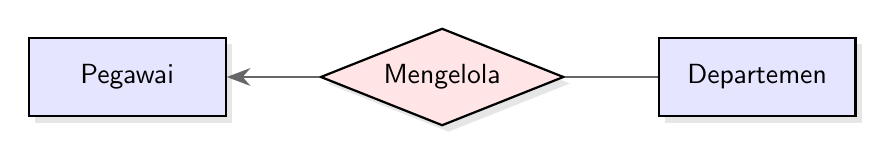
\begin{tikzpicture}[
			entity/.style={draw, rectangle, minimum width=2.5cm, minimum height=1cm, fill=blue!10, thick, font=\sffamily, drop shadow={opacity=0.2}},
			relation/.style={draw, diamond, aspect=2.5, minimum width=3cm, minimum height=1.2cm, fill=red!10, thick, font=\sffamily, drop shadow={opacity=0.2}},
			line/.style={thick, color=gray!80!black}
		]
		\node[entity] (pegawai) at (-4,0) {Pegawai};
		\node[entity] (dept) at (4,0) {Departemen};
		\node[relation] (mengelola) at (0,0) {Mengelola};

		\draw[line, -{Stealth[length=3mm]}] (mengelola.west) -- (pegawai.east);
		\draw[line] (mengelola.east) -- (dept.west);
	\end{tikzpicture}
	\caption{Relasi Many-to-One dengan Tanda Panah "Paling Banyak Satu" pada Sisi Pegawai.}
	\label{fig:cardinality}
\end{figure}

\section{Batasan Partisipasi (Participation Constraints)}

Selain kardinalitas, kita juga harus mendefinisikan aturan partisipasi entitas di dalam sebuah relasi. Terdapat dua jenis partisipasi:

Pertama, \textbf{Partisipasi Total} (Total Participation), yang digambarkan dengan dua garis sejajar. Ini berarti setiap entitas dalam himpunan tersebut \textit{wajib} berpartisipasi dalam relasi. Contoh: Sebuah entitas "Pinjaman" (uang) tidak mungkin ada di dunia nyata tanpa ada "Customer" yang meminjamnya. Maka, partisipasi Pinjaman dalam relasi Peminjaman adalah total.

Kedua, \textbf{Partisipasi Parsial} (Partial Participation), digambarkan dengan satu garis. Ini berarti beberapa entitas mungkin tidak berpartisipasi dalam relasi tersebut. Contoh: Tidak semua "Customer" harus memiliki "Pinjaman" (mungkin ia hanya punya tabungan).

\section{Entitas Kuat vs Entitas Lemah}

Sebuah entitas dikatakan \textbf{Entitas Kuat} (\textit{Strong Entity}) jika ia memiliki cukup atribut untuk membentuk Primary Key-nya sendiri (contoh: Pegawai dengan NIP).

Sebaliknya, \textbf{Entitas Lemah} (\textit{Weak Entity}) adalah entitas yang tidak memiliki Primary Key sendiri. Keberadaannya sangat bergantung pada entitas lain (entitas kuat). Contoh klasik adalah entitas "Pembayaran" pada sebuah "Pinjaman". Sebuah pembayaran tidak akan pernah ada jika tidak ada pinjaman.

Pada Gambar \ref{fig:weak}, entitas lemah digambarkan dengan persegi panjang bersusun dua (\textit{double rectangle}). Hubungannya dengan entitas kuat digambarkan dengan belah ketupat bersusun dua yang disebut relasi pengidentifikasi (\textit{Identifying Relationship}). Primary key dari entitas lemah didapat dari kombinasi Primary Key entitas kuat ditambah dengan \textit{Discriminator} (garis bawah putus-putus) miliknya sendiri. Jadi, Primary Key untuk Pembayaran adalah (no-pinjam, no-byr).

\begin{figure}[H]
	\centering
	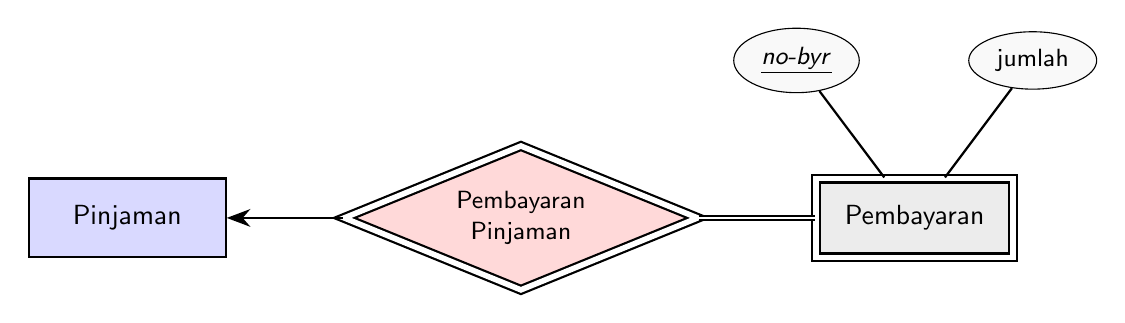
\begin{tikzpicture}[
			strong/.style={draw, rectangle, minimum width=2.5cm, minimum height=1cm, fill=blue!15, thick, font=\sffamily},
			weak/.style={draw, rectangle, double, double distance=2pt, minimum width=2.5cm, minimum height=1cm, fill=gray!15, thick, font=\sffamily},
			ident/.style={draw, diamond, double, double distance=2pt, aspect=2, minimum width=4.5cm, minimum height=1.2cm, fill=red!15, thick, font=\small\sffamily, align=center}
		]
		\node[strong] (pinjam) at (0,0) {Pinjaman};
		\node[weak] (bayar) at (10,0) {Pembayaran};
		\node[ident] (rel) at (5,0) {Pembayaran\\Pinjaman};

		\node[draw, ellipse, fill=gray!5, font=\small\sffamily] (nobyr) at (8.5,2) {\underline{\textit{no-byr}}};
		\node[draw, ellipse, fill=gray!5, font=\small\sffamily] (jml) at (11.5,2) {jumlah};

		\draw[thick] (bayar) -- (nobyr);
		\draw[thick] (bayar) -- (jml);

		\draw[thick, -{Stealth[length=3mm]}] (rel.west) -- (pinjam.east);
		\draw[thick, double] (rel.east) -- (bayar.west);
	\end{tikzpicture}
	\caption{Representasi Entitas Lemah (Pembayaran) dan Relasi Pengidentifikasinya.}
	\label{fig:weak}
\end{figure}

\section{Kesimpulan}

Entity Relationship Diagram (ERD) adalah seni menerjemahkan kebutuhan bisnis yang rumit menjadi sebuah peta visual yang terstruktur. Melalui pemahaman terhadap anatomi entitas, atribut, relasi, hirarki kunci, kardinalitas, batasan partisipasi, hingga entitas lemah, seorang perancang basis data dapat membangun fondasi yang kokoh. ERD bukanlah sekadar gambar, melainkan kontrak konseptual yang memastikan bahwa data yang akan disimpan nantinya benar-benar merepresentasikan realitas bisnis secara akurat, efisien, dan bebas dari anomali.

\newpage
\section*{Referensi}
\addcontentsline{toc}{section}{Referensi}

\begin{thebibliography}{99}
	\bibitem{lubis}
	Lubis, A. I. (2026). \textit{Entity Relationship Diagram} [Slide Presentasi Mata Kuliah Pengantar Basis Data]. Politeknik Negeri Batam.

	\bibitem{silberschatz}
	Silberschatz, A., Korth, H. F., \& Sudarshan, S. (2019). \textit{Database System Concepts} (7th ed.). McGraw-Hill Education.
\end{thebibliography}

\end{document}
